\documentclass[consecutivenumbering]{gadsescript}

\KOMAoption{toc}{indent}
\DeclareTOCStyleEntry[indent = 0cm, entryformat=\normalfont\bfseries, pagenumberformat=\normalfont\bfseries]{tocline}{section}

\usepackage{hyperref}

\settitle{Analysis I}
\setfaculty{Faculty of Science (Mathematics and Statistics)}
\setuniversity{University of Konstanz}
\setsemester{Winter Semester 2023/2024}

\begin{document}
\maketitle

\tableofcontents
\newpage

\section*{Organisation, Tipps \& Tricks und Literaturhinweise}

Mathe...
\begin{itemize}
	\item ist intellektuell extrem herausfordernd
	\item kommt mit einem hohen Arbeitsaufwand
	\item oft falschen Erwartungen und
	\item ist wie Ausdauersport
\end{itemize}

aber dafür ist Mathe eines der  schönsten Studien c:

Generelles Zeitmanagement:
\begin{itemize}
	\item Vor- und Nachbereitung wahrscheinlich mehr als die gesetzten $14 \times \qty{3}{\hour} = \qty{42}{\hour}$
	\item Klausurvorbereitung auch mehr als $\qty{39}{\hour}$
	\item Pro Woche $ 2 \times \qty{1.5}{\hour}$, $2 \times \qty{2}{\hour} $, $ \qty{1.5}{\hour} $, $ \qty{10}{\hour} $
	\item Es gibt immer eine Aufgabe die man nicht lösen kann
	\item In die Vorlesungen kommen
\end{itemize}

Vorlesung:
\begin{itemize}
	\item normal nicht alles zu verstehen
	\item Notizen was man nicht versteht
	\item Punkte konzise angehen
	\item \textbf{Mathe muss sich gedanklich setzen} - genügend Zeit zu verarbeiten
\end{itemize}

Übungen:
\begin{itemize}
	\item zeitintensiv
	\item Ergebnisse vernünftig aufschreiben
	\item Weg zu einer korrekter Lösung ist sehr langwierig
	\item \textbf{nicht 10 Blätter Papier ab, von denen 9.5 inkonklusiv sind}
	\item also schön Aufschreiben
\end{itemize}

Wenn wir einen Satz gezeigt bekommen, dann bekommen wir nicht die gescheiterten Jahrelangen Versuche zur Schau, sondern nur die Ausgearbeitete Lösung $\rightarrow$ also bei uns auch langer weg, aber Aufschreiben nur klein

Übungszettel:
\begin{itemize}
	\item $ 50\% $ muss richtig sein
	\item bis Freitag 10:00 Uhr
	\item in F4
	\item diese Woche nicht so umfangreich, weil weniger Zeit
	\item auf ILIAS Terminfindung Abstimmung
	\item Donnerstag Einteilung in Tutorien
	\item Blätter tackern :c
	\item alle zwei Wochen Beweismechanik Aufgaben, nur digital nicht in Papier (ist dann die letzte Aufgabe)
\end{itemize}

Literaturempfehlung:
\begin{itemize}
	\item Otto Forster: Analysis 1
		\begin{itemize}
			\item kurz und knapp - aber konzise, udn das hilft
			\item ähnliche Struktur wie Vorlesung
			\item weig motivation und wenige Querverbindungen
		\end{itemize}
	\item Königsberger: Analysis 1
		\begin{itemize}
			\item kurz - aber konzise
			\item alle themen der Vorlesung, andere Struktur
			\item mehr motivation und Querverbindungen
		\end{itemize}
	\item Klaus Fritsche: Grundkurs Analysis 1
		\begin{itemize}
			\item ausführlich
		\end{itemize}
	\item Daniel Grieser: Analysis I
		\begin{itemize}
			\item Ausfühlich, aber mit Fokus auf das Wesentliche
			\item alle Themen der Volesung enthalten, ähnliche Struktur
			\item bunt??
		\end{itemize}
	\item Harro Huser: Lehrbuch der Analysis Teil 1
		\begin{itemize}
			\item extrem ausfühlich,dick, an einigen stellen sehr extensiv
			\item alle und mehr Themen als Vorlesung
			\item Querverbindungen
		\end{itemize}
	\item Walter Rudin: Analysis
		\begin{itemize}
			\item sehr knapp und elegant
			\item klassiker
			\item alle themen der Volesung, leicht andere Struktur
			\item empfehlenswertes Buch fortgeschrittene Leser*innen
			\item nicht für Anfänger*innen
		\end{itemize}
	\item Herber amann, Joachim Escher: Analysis I
		\begin{itemize}
			\item strkt logischer Aufbau, damit teils länglich. Großes Bild
			\item alle Themen, andere Struktur
			\item auch nicht für anfänger*innen
		\end{itemize}
	\item Terence Tao: Analysis (englisch, aber gut)
	\item Rober Denk, Reinhard Racke: Kompendium der ANalysis
		\begin{itemize}
			\item kurz und knapp, teils wie Nachschlagewerk
			\item alle themen
		\end{itemize}
	\item Florian Modler, Martin Kreh: Tutorium Analysis 1 und Lineare Algebra 1
		\begin{itemize}
			\item kurz und knapp, teils wie nachschalgewerk
			\item von studierende für studierende
			\item aber enthält ein paar Fehler
		\end{itemize}
\end{itemize}

\newpage
\section{Natürliche Zahlen und elemntare Begriffe}
\subsection{Zahlbereiche}
\[ \N \coloneqq \{ 1, 2, 3, \dotsc \} \]
\[ \N_0 \coloneqq \{ 0, 1, 2, 3, \dotsc \} \]
\[ \Z \coloneqq \{ \dotsc, -3, -2, -1, 0, 1, 2, 3, \dotsc \} \]
\[ \Q \coloneqq \{ \frac{p}{q} : p \in \Z, q \in \N \} \]
\[ \R \coloneqq \{ \text{ reelle Zahlen } \} \]

Wir besprechen gar nicht was eine Menge ist, das ist zu philosophisch\\
Es ist schwierig Mengen zu Definieren, man kommt schnell auf logische Wiedersprüche

\begin{itemize}
	\item Notation: für $ x $ schreiben wir für eine Eigenschaft $ A $ ``$ A(x)$'', falls $ x $ $ A $ erfüllt.
	\item[$\rightarrow$] Menge aller Objekte $ x $ mit $ A(x) $
		\[ \{ x : A(x) \} \]
	\item[$\rightarrow$] gibt es kein $ x$ mit $ A(x) $, so nennen wir die Menge leer, ``$\emptyset$''
\end{itemize}

\begin{itemize}
	\item $\exists \hat= \text{ Existenzquantor, ``es existiert''}$
	\item $ A, B, $ Eig., $M\coloneqq \{ x : x \text{ erf. } A \}$\\
		$N \coloneqq \{ x : \text{ erf. } B \} $\\
	$ M \subset N$, falls $ \forall x \in M : x \in N $
	\item $ M = N $, falls $ M \subset N \vee N \subset M $
	\item ``Echte Tielmenge'': $ M \nsubseteqq N$, falls $ M \subset N, N \neq N.$
\end{itemize}

\begin{subexample}[(gerade Zahlen)]
	$ n \in \N_0 \text{ gerade } :\iff ( \exists k \in \N_0 : n = 2k) $
	\begin{align}
		M \coloneqq &\{ n \in \N_0 : \exists k \in \N_0 : n = 2k \}\\
		=&\{2k : k \in \N_0
	\end{align}
\end{subexample}

\begin{example}[$ \N \subsetneqq \N_0 \subsetneqq \Z \subsetneqq \Q \subsetneqq \R $]
	Zu $ \Q \subsetneqq \R : \sqrt{2} \notin \Q $. Widerspruchsbeweis: Ang.,
	$ \sqrt{2} \in \Q $, so $ \sqrt{2} = \frac{p}{q} $, mit $ p \in \N_0, q \in \N $. \OE $ p, q $ teilerfremd (d.h. Bruch ist vollständig gekürzt).. Also $ p^2 = 2q^2 $\\
	$\implies$ $ p $ ist gerade. Also $ p = 2l $ mit $l \in N_0$.\\
	$\implies$ $ 4l^2 = p^2 = 2q^2 \implies 2l^2 = q^2 \implies q $ gerade.\\
	$ \implies $ $ p, q $ gerade. $ \implies p, q $ nicht teilerfremd. \qed
\end{example}

\subsection{Vollständige Induktion}
\begin{itemize}
	\item Ziel: Beweis von Aussagen für alle $ n \in \N_0 $
\end{itemize}
\textbf{Dominoprinzip}: Wenn alle Steine umfallen sollen,
\begin{itemize}
	\item müssen wir den 1. Stein umwerfen,
	\item muss stehts der $n$-te Stein den $(n+1)$-ten umwerfen.
\end{itemize}

\textbf{Prinzip (vollst. Ind.)} Wollen wir eine Aussage $ A(n) \forall n \in \N $ zeigen; so zeigen wir
\begin{enumerate}[label=(\roman*)]
	\item $ A(1) $ gilt (Induktionsanfang)
	\item Aus $ A(n) $ für $ n \in \N $ stets $ A(n+1) $ folgt. (Induktionsschritt)
\end{enumerate}

\begin{definition}[Summen]
	Für $x_-1, \dotsc, x_n \in \R $ definieren wir
	\[ \sum_{k = 1}^{n} x_k \coloneqq x_1 + \dotsc + x_n \]
\end{definition}

\begin{example}[Geometrische Summe]
	\[ \forall n \in \N : \]
	\begin{equation}
		\underbrace{\sum_{k=0}^{n} x^k}_{x^0 + x^1 + ... + x^n} =  \frac{1-x^{n+1}}{1-x}
	\end{equation}
	
	\begin{description}
		\item[I.A. $n = 1$]
			\[ \sum_{k=0}^{1}x^k = x^0 + x^1 = 1+x = \frac{(1-x)(1+x)}{1-x} = \frac{1-x^2}{1-x} \]
		\item[I.S.]
			\[ n \to n+1 \] Angenommen, (equation) gilt für ein $n \in \N $.
			z.z. (equation) gilt für $ n + 1 $
			\[ \sum_{k=0}^{n+1}x^k = \left( \sum_{k=0}^{n}x^k\right) + x^{n+1} =  \frac{1 - x^{n + 1}}{1 - x} + x^{n + 1}\]
			...
	\end{description}
\end{example}

\begin{example}[Für welche $ n \in \N $ gilt $ n^2 < 2^n $?]
	\begin{itemize}
		\item $n = 1 \to 1 < 2$\\
			$ n = 2 \to n^2 = 4 \nless 4 = 2^2 $\\
			$ n = 3 \to n^2 = 9 \nless < 2^3 $\\
			$ n = 4 \to n^2 = 16 \nless 16 = 2^4 $\\
			$ n = 5 \to n^2 25 < 32 = 2^5 $
	\end{itemize}

	Wir versuchen die Aussage $ \forall n \geq 5 $ zu zeigen.

	\begin{description}
		\item[I.A.:] $ n = 5 : n^2 = 25 < 32 = 2^5 $
		\item[I.S.:] Ang., Aussage gilt für $ n \geq 5 $. Wir müssen zeigen:
			\[ ( n + 1 )^2 < 2^{n + 1} \]
			$ ( n + 1 ) ^2 = \underbrace{n^2}_{<2^n} + 2n + 1 < 2^n + 2n + 1 \mid \overset{?}{<} 2^{ n  + 1} $
			Angenommen, es gilt 
			\begin{equation}
				\label{eq:heart} \forall n \geq 5 : 2n + 1 < 2^n
			\end{equation}
			Dann: $ ( n + 1)^2 < ... < 2^n + 2n + 1 = 2 * 2^n = 2^{n+1} $
			\begin{itemize}
				\item Wir zeigen (\ref{eq:heart}) wiederum mit voll. Ind.
					\begin{description}
						\item[I.A.:] $ n = 5 2n + 1 = 11 < 32 = 2^5 $
						\item[I.S.:] Ang., (\ref{eq:heart}) gilt für $n \in \N $. Dann gilt:
							$ 2(n+1) + 1 = 2n + 3 = (2n + 1) + 2 < 2^n + 2 < 2^n + 2^n = 2*2^n = 2^{n+1} $.\\
							Damit folgt (\ref{eq:heart} und damit die eigentliche Aussage \qed
					\end{description}
			\end{itemize}
	\end{description}

\end{example}

\begin{definition}
	für $ n \in \N_0 $ definieren wir die \textit{Fakultät} via $n! \coloneqq n \times (n-1) \times \dotsb \times 2 \times 1 $, falls $n \geq 1 $, und $0! \coloneqq 1 $.
	Für $ k \in \{ 0, \dotsc, n\} $ definieren wir den \textit{Binomialkoeffizienten}
	\[ \binom{n}{k} \coloneqq \frac{ n!}{k!(n-k)!}.\]
\end{definition}

\begin{lemma}
	Für alle $ n \in \N $ und alle $ k \in \{ 1, \dotsc, n \}: $
	\[ \binom{n}{k} + \binom{n}{k-1} = \binom{ n+1}{k}\]
	\begin{proof*}
		\begin{align*}
			\binom{n}{k} + \binom{n}{k-1} &= \frac{n!{\color{yellow}(n-k+1)}}{k! (n-k)!{\color{yellow} (n-k+1)}} + \frac{n!{\color{yellow}(k)}}{(k-1)! (n-(k-1)k)!{\color{yellow} (k)}}\\
			= \frac{n!n + n!}{k!(n-k+1!} &= \frac{n!(n+1)}{k!(n-k+1)!} \qed
		\end{align*}
	\end{proof*}
\end{lemma}

\begin{example}[(Binomische Formel)]
	Für $ x, y \in \R $ und $ n \in \N_0 $:
	\[ (x+y)^n ? \sum_{k=0}^{n} \binom{n}{k}x^ky^{n-k}. \]
	Sei also $ x, y \in \R $.
	\begin{description}
		\item[I.A.:] $n=0$. $(x+y)^0 = 1 = \binom{0}{0} x^0y^0 $
		\item[I.S.:] Gelte die Aussage für $ n \in \N_0 $
			\begin{align}
				\label{eq:3}
				(x+y)^{n-1} = (x+y)(x+y)^n &= (x+y)\sum_{k=0}^{n}\binom{n}{k}x^ky^{n-k}\\
				~&= x\sum_{k=0}^{n}\binom{n}{k}x^ky^{n-k} + y\sum_{k=0}^{n}\binom{n}{k}x^ky^{n-k}\\
				\label{eq:7}~&=\sum_{k=0}^{n}\binom{n}{k}x^{k+1}y^{n-k} + \sum_{k=0}^{n}\binom{n}{k}x^ky^{n+1-k}
			\end{align}
			Indexverschiebung: $ l = k+1 $. $l \in \{ 1, \dotsc, n+1\} $
			\begin{align*}
				(\ref{eq:7}) &=\underbrace{\sum_{l=1}^{n}\binom{n}{l-i}x^ly^{n+1-l}}_{\text{Hier Indexverschiebung}} + \underbrace{\sum_{l=0}^{n}\binom{n}{l}x^ly^{n+1-l}}_{\text{Hier nennen wir einfach $ k = l $}}\\
				~&= \binom{n}{n}x^{n+1}y^0 + \left(\sum_{k=0}^{n}\left(\binom{n}{l-1}+\binom{n}{l}\right)x^ly^{n+1-l} \right) + \binom{n}{0}x^0 y^{n+1}\\
				~&= \binom{n+1}{n+1}x^{n+1}y^{0} + \left( \sum_{l=1}^{n}\binom{n+1}{l}x^ly^{(n+1)-l} \right) + \binom{n+1}{0}x^0y^{n+1}\\
				~&= \sum_{l=0}^{n+1} \binom{n+1}{l} x^ly^{(n+1)-l} \qed
			\end{align*}
	\end{description}
\end{example}

\subsubsection{Characterisierung der natürlichen Zahlen}
\begin{subdefinition}
	Eine Teilmenge $ M \subset \R $ heißt induktiv, falls
	\begin{enumerate}[label=(\roman*)]
		\item \label{en:1}$ 1 \in M $
		\item \label{en:2}$ \forall x \in M : x + 1 \in M $
	\end{enumerate}
	\begin{subexample}
		\begin{enumerate}[label=(\alph*)]
			\item $ \N $ sind ind. Menge.
			\item $ A \coloneqq \{ 2n : n \in \N_0 \} $ nicht ind. Menge, da \ref{en:1} $ 1 \neq A $, \ref{en:2} $2n + 1 $ ist immer ungerade
			\item $ B \coloneqq \{ 2n + 1 : n \in \N_0 \} $ nicht ind.: \ref{en:1}, aber $ 2n + 1 + 1 = 2 (n+1) $
			\item $\Q^+ \coloneqq \{ x \in \Q: q > 0 \} $ ist ind. Teilmenge
		\end{enumerate}
	\end{subexample}
\end{subdefinition}
\begin{itemize}
	\item Sei $ (A_i)_{i\in I} $ mit I Indexmenge eine Familie von Mengen. setze
		\[ \bigcap_{i\in I} \coloneqq \{ x : (\forall i \in I: x \in A_i ) \}\quad\text{Schnitt} \]
		\[ \bigcup_{i\in I} \coloneqq \{ x : ( \exists i \in I: x \in A_i ) \}\quad\text{Vereinigung} \]
\end{itemize}

\begin{subproposition}
	Für eine Menge $ M \subset \R $ sind äquivalent
	\begin{enumerate}[label=(\roman*)]
		\item \label{en:4}$ M = \N $
		\item \label{en:5}Ist $ N \subset \R $ induktiv, so $ M \subset N $
		\item \label{en:6}\[ M = \bigcap_{N\subset\R} N \text{ induktiv} \]
	\end{enumerate}

	$\ref{en:4} \iff \ref{en:5} \iff \ref{en:6}$
	\begin{subproof*}
		\begin{description}
			\item[`$\ref{en:4} \implies \ref{en:5}$':] Sei $ N \subset \R $ beliebige ind. Teilmengen von $\R$. Zu zeigen: $ M \overset{\ref{en:4}}{=} \N \subset N $\\
			Aber $ 1 \in \N $, und $ 1 \in N $ (da $ N $ ind. ), Da $ N $ ind. ist, ist mit jeder nat. $ x \in \N $ also auch $ x \in N $. Damit $ x + 1 \in \N $ \fbox{$\N \subset N.$}

		\item[`$\ref{en:5} \implies \ref{en:6}$'] Wir zeigen: \[\bigcap_{N \text{ ind. Menge}} N \] ist ind. Menge\\
			$\overset{\ref{en:5}}{\implies} M \overset{\ref{en:5}}{\subset} N \subset M $. Also \[ M = \bigcap_{N \text{ ind.}} N. \]
				\[\bigcap_{N \text{ ind}} N \text{ induktiv:}\]
				\begin{enumerate}[label=(\roman*)]
					\item \[ ( \forall N \text{ ind: } 1 \in N) \implies 1 \in \bigcap_{N \text{ ind.}} N \]
					\item \[ \forall x \in \R : x \in \bigcap_{ N \text{ ind.}} N \left( \implies x \in \bigcap_{N \text{ ind.}} N \right) \overset{\text{DEF.}}{\implies} \forall N \text{ ind.} : x + 1 \in N \implies x + 1 \in \bigcap_{N \text{ ind.}}\]
				\end{enumerate}
			\item['$\ref{en:6} \implies \ref{en:4}$'] Noch zu zeigen (blöd glaube ich oder ÜA, wir hatten auf jeden Fall keine Zeit in der Vorlesung) \qed
		\end{description}
	\end{subproof*}
\end{subproposition}

\section{Körper}
\subsection{Was sind Strukturen?}
\subsection{Körper}
\begin{subdefinition}[Körper]
	in script of Prof. and on paper
\end{subdefinition}
\begin{subexample}
	in script of Prof. and on paper
\end{subexample}
\begin{subexample}
	in script of Prof. and on paper
\end{subexample}
\begin{sublemma}
	in script of Prof. and on paper
\end{sublemma}
\begin{sublemma}
	in script of Prof. and on paper
\end{sublemma}
\begin{tabular}{cc}
	$\Q$ & $\R$\\
	$\uparrow $ & $\uparrow $\\
	abzählbar & nicht abzählbar\\
\end{tabular}
Kontinuumshypothese
\hrule
\begin{definition}
	In der Situation von definition \ref{2.2.1} sei $ n \in \N $, sowie $ x_1, \dotsc, x_n \in K $. Wir definieren rekursiv $ x_1 + \dotsb + x_n \coloneqq ( x_1 + \dotsb + x_{n-1} ) + x_n, x: \cdot \dotsb \cdot x_n \coloneqq ( x_1 \cdot \dotsb x_{n-1} ) \cdot x_n $
\end{definition}
\begin{definition}
	In der Situation von Definition \ref{2.2.1} sei $ n \in \N_0 $ und $ x \in K $. Wir definieren
	\[ x^0 \coloneqq 1_K \text{ und } x^n \coloneqq ( x^{n-1} \cdot x, n \in \N \]
	Ist $ x \in K\setminus\{0\} $, so sei für $ n \in \N : x^{-n} \coloneqq ( x^{-1})^n $.
\end{definition}
\begin{lemma}
	Für alle $ x, y \in K, \quad m, n \in \N_0 $:
	\begin{enumerate}[label=\roman*)]
		\item $x^n\cdot x^m = x^{n+m}$,
		\item $(x^n)^m = x^{n\cdot m} $,
		\item $ x^n \cdot y^n = ( x \cdot y ) ^n $
	\end{enumerate}
	Ist zudem $ x, y \neq 0_K $, so gelten diese Identitäten auch für $n,m \in \Z $
	\begin{proof*}[i]
		Fixiere $ n \in \N_0 $, nun Induktion nach $m$.
		\begin{description}
			\item[I.A.] $m = 0$. $x^n\cdot x^0 \overset{\text{Def.}}{=} x^n \cdot 1_K \overset{\text{(M2)}}{=} 1_K \cdot x^n \overset{\text{(M3)}}{=} x^n= x^{n+0} $
			\item[I.S.] Gelte die Aussage für ein $m \in \N_0$. Zeige für $ m \curvearrowright m+1 $
				\[ x^n \cdot x^{m+1} \overset{\text{Def.}}{=} x^n\left(x^m) \cdot x\right) \overset{\text{(M1)}}{=} \left( x^n\cdot x^m\right) \cdot x \overset{\text{IV}}{=} x^{n+m} \cdot x \overset{\text{Def.}}{=} x^{n+m+1} \qed \]
		\end{description}
	\end{proof*}
\end{lemma}

\subsection{Angeordnete Körper}
\begin{itemize}
	\item Ziel Vergleich von Elementen hinsichtlich ``Größe''
\end{itemize}
\begin{subdefinition}
	Eine \textbf{Relation} auf einer Menge $M$ ist eine Teilmenge $ R\subset M\times M $. Ist $ ( x, y ) \in R $, so schreiben wir auch $xRy$ oder $ R(x,y) $ und sagen, dass $x $ und $ y $ über $ R $ in Relation stehen.
\end{subdefinition}
\begin{subexample}
	$ M = \text{ Stidierende im Hörsaal,}$\\
	$ (x,y) \in M \times M : x R y :\iff x $ kennt den Namen von $ y $
	\begin{itemize}
		\item $ R $ \textbf{reflexiv}? (d.h. $\forall x \in M : x R y ) $\qquad Ja
		\item $ R $ \textbf{symmetrisch}? ( d.h. $\forall x, y \in M : x R y \iff y R x ) $ ) \qquad Nein
		\item $ R $ \textbf{transitiv}? ( d.h. $ \forall x, y, z \in M : xRy \wedge yRx \implies xRz $ ) \qquad \textbf{Nein}
	\end{itemize}
\end{subexample}
\begin{subdefinition}
	Sei $ R $ eine Relation auf einem Kürper $ K $. $ R $ heiß \textbf{Ordnung} auf $ K $, falls gilt
	\begin{enumerate}[label=(\roman*)]
		\item \textbf{Trichotomie:} $ \forall x \in K: $ Entweder $ 0_K Rx, x R0_K $ oder $ x = 0_K $
		\item \textbf{Abgeschlossenheit bezüglich Addition} $ \forall x,y \in K : 0_K R x, 0_K R y \implies 0_K R (x+y)$
		\item \textbf{Abgeschlossenheit bezüglich Multiplikation} $ \forall x, y \in K: 0_K R x, 0_KRy \implies 0_K R (x\cdot y) $
	\end{enumerate}
	Das Tupel $ ( K, R ) $ heißt \textbf{angeordneter Körper.} (\textbf{Schreibe} auch `$<$' für  $ R $).
	\begin{description}
		\item[Setze für $a,b \in K $:]
			\begin{align*}
				a < b &:\iff 0_K < ( b- a )\\
				a > b &:\iff b < a\\
				a \leq b &:\iff a < b \vee a = b\\
				b \geq a &:\iff a \leq b\\
			\end{align*}
	\end{description}
\end{subdefinition}

\begin{sublemma}
	Sei $ ( K, < ) $ angeordneter Körper, $ a, b, c \in K $
	\begin{enumerate}[label=(\roman*)]
		\item Entweder $ a > b, a = b \vee a < b $.
		\item $ a < b \wedge b < c \implies a < c $
		\item $ ( a > 0 \implies (-a) < 0) \wedge ( a < 0 \implies (-a) > 0) $
		\item Gilt $ a < b $, so ist
			\begin{align*}
				ac < bc, & \qquad c>0\\
				ac > bc, & \qquad c < 0\\
				a^2 > 0, & \qquad a \neq 0\\
			\end{align*}
			\[ a > 0 \implies a^{-1} > 0 \]
			\[ a < 0 \implies a^{-1} < 0 \]
			$ b^{-1} < a^{-1} $, falls $ a > 0 $\\
			$ a + c < b + c $.
		\item $ a < b \implies (-a) > (-b) $
	\end{enumerate}
	\begin{subproof*}[(i)-(iii)]
		\begin{enumerate}[label=(\roman*)]
			\item Da $ a < b \iff 0_K < b - a $, folgt das aus Trichotomie und Def. von `$>$'.
			\item zu zeigen: $ a y c $, d.h. $ 0_K < c-a$.
				\[ c - a = ( c + 0_K ) - a = \underbrace{(c-b)}_{>0} + \underbrace{(b-a)}_{>0} > 0, \text{ d.h. } a < c \]
			\item $ a > 0 $. Angenommen, $ (-a ) > 0. \overset{\text{Abg. Add.)}}{\implies} 0_K = a + (-a) > 0_K \overset{\text{Trich.}}{\implies} \Lightning $ Ist $-a = 0$, so $ a = 0 $, nach Trich. Wid. zu $ a > 0 $. Falls $ a < 0 $, analog.\qed
		\end{enumerate}
	\end{subproof*}
\end{sublemma}
\begin{subcorollary}
	Es gibt keine Ordnung `$<$' auf $\F_2$, die $\F_2$ zu einem angeordneten Körper macht
	\begin{proof*}
		Angenommen, `$<$' sei Ordnung. Da $ 0_K \neq 1_K $, gilt entweder $ 0_K < 1_K $ oder $ 1_K < 0_K $ (nach Trich.). Falls $ 0_K < 1_K $. Dann $ 0_K = 1_K + 1_K $ damit $ 0_K = 1_K + 1_K > 0_K + 1 = 1_K $. Widerspruch für $1_K < 0_K$ argumentiere analog.
	\end{proof*}
\end{subcorollary}
\begin{itemize}
	\item \textsc{Prinzip:} $\R \wedge \Q $ sind angeordnete Körper
\end{itemize}

\subsection{Der Betrag}
(`Abstand zur Null')
\begin{subdefinition}
	Für $ x \in \R $ definieren wir den Betrag $|x| \coloneqq \begin{cases}x,&x\geq0,\\-x,&x<0\end{cases}$
\end{subdefinition}
\begin{sublemma}
	Der in Def 2.4.1 eingeführte Betrag erfüllt
	\begin{enumerate}[label=(\roman*)]
		\item $ forall x \in \R |x| \geq 0$
		\item $  |x| = 0 \iff x = 0 $
		\item Multiplikativität: $ \forall x,y \in \R : | x\cdot y | = | x | \cdot | y | $
		\item {\color{yellow} \textbf{Dreiecksungleichung:} $ \forall x, < \in \R: | x + y | \leq | x | + | y |$ }
		\item $ \forall x \in \R : | -x| = | x | $
		\item $ \forall x, y \in \R :  y \neq 0 \implies \left| \frac{x}{y} \right| = \frac{|x|}{|y|} $
	\end{enumerate}
\end{sublemma}

\subsection{Das Archimedische Axiom}
\textsc{Prinzip}-Arch. Axiom: $ \forall x \in \R, x > 0 \exists n \in \N : x < n $\\
.\qquad.\qquad.\qquad.\qquad.\qquad.\quad$\underset{x}{|}$ $\underset{n}{.}$
\begin{itemize}
	\item Das muss gefordert werden
\end{itemize}

\subsection{Supremum, Infimum und die Supremumseigenschaft}
\begin{itemize}
	\item \textbf{Ziel}: Entscheidende Eigenschaft von $\R$
\end{itemize}
\begin{subdefinition}
	Eine nichtleere Teilmenge $ A \subset \R $ heißt
	\begin{itemize}
		\item \textbf{nach oben beschränkt}, falls $\exists c \in \R \forall x \in A: x \leq c $. Ein solches c ``obere Schranke''
		\item \textbf{nach unten beschränkt}, falls $ \exists c \in \R \forall x \in A: c \leq x $ `` untere Schranke''
	\end{itemize}
\end{subdefinition}

\begin{subexample}
	\begin{itemize}
		\item $ A = N_0 $ durch $ 0 $ nach unten, nach oben unbegrenzt
		\item $ A = \{ 1, 2, \dotsc, 10\} $ durch $ 1 $ nach unten, und durch $ 10, 11, \dotsc $ nach oben beschränkt
	\end{itemize}
\end{subexample}

\begin{subdefinition}
	Sei $ a \subset \R $ nichtleer
	\begin{enumerate}[label=(\roman*)]
		\item Ist $ A $ nach oben beschränkt, so heißt $ s ( \eqqcolon \operatorname{sup}A) $ \textbf{Supremum} von $ A $, falls $ s $ obere Schranke ist \textit{und} \textbf{kleinste obere Schranke} ist d.h. $ \forall c \in \R : c $ obere Schranke von $ A \implies s \leq c $. Ist $ s \in A $ Supremum von $ A $, so heißt $ s $ \textbf{Maximum} von $ A $.
		\item Ist $ A $ nach oben unbeschränkt, so sei $ + \infty $ das Supremum von $ A $.
		\item Ist $ A $ nach unten beschränkt, so nennen wir $ s^\prime \in \R $ \textbf{Infimum} von $ A $, falls $ s^\prime$ untere Schranke und für jede andere untere Schranke $ d \in \R $ von $ A $: $ d \leq s^\prime $. Ist $ s^\prime \in A $ Infimum, so heißt $ s^\prime $ \textbf{Minimum} von $ A $.
		\item Ist $ A $ nach unten unbeschränkt, so sei $ - \infty $ das Infimum von $ A $
	\end{enumerate}
	\textbf{Schreibweise}: $ \sup(A), \max(A), \inf(A), \min(A)$.
\end{subdefinition}

\begin{subexample}
	Für $ a, b \in \R $ mit $ a y b $ sei $ ( a, b ) \coloneqq \{ \R : a < x < b \} $\\
	Dann: $ \sup((a,b)) = b \wedge \inf((a,b)) = a $.
	\begin{itemize}
		\item Obere Schranke: $ \forall x \in (a,b) : x <  ) \implies b $ obere Schranke.
		\item Ist $ d $ andere obere Schranke, so $ b \leq d $. Klar: $ d > a $, also angenommen $ a < d < b $.\\
			Dann $ x \coloneqq \frac{d+b}{2} \in ( a, b), x > d. \implies d $ keine obere Schranke \Lightning\\
			Weiter $ b \notin (a, b) $, also $ b $ Supremum, kein Maximum
	\end{itemize}
\end{subexample}

\fbox{\textsc{Prinzip}} (Supremumseigenschaft)\\
Jede nach oben beschränkte Menge $ A \subset \R $ hat ein Supremum in $ \R $
\textbf{Informell}: $ ( 1, \sqrt{2} ) \cap \Q $ hat $\sup = \sqrt{2} $ (später). Aber $ \sqrt{2} \notin \Q $, also gilt die Supremumseigenschaft für $ \Q $ nicht.\par

$ \R $ ist
\begin{itemize}
	\item Körper
	\item angeordente Körper
	\item bewerteter Körper
	\item Archimedisch angeordnete Körper
	\item \textbf{Supremumseigenschaft}
\end{itemize}

\section{Folgen und Konvergenz}
\subsection{Reele Folgen und Konvergenz}
Folge $ a: \N \ni n \mapsto a ( n ) \in \R $. Schreibweisen:
\[ ( \underbrace{a_n}_{( = a(n))} )_{n \in \N} \text{( $ n $ Laufindex)}, (a_n) \]
\begin{subexample}
	\[ a_n \coloneqq 2  n \to \text{ Folge der geraden Zahlen} \]
	\[ a_n \coloneqq 2n+1 \to \text{ Folge der ungeraden Zahlen} \]
\end{subexample}

\begin{subdefinition}[Konvergenz]
	Sei $ (a_n) $ eine Folge in $ \R $ $ ( ( a_n ) \subset \R ) $ und $ a \in \R $. Wir sagen, dass $ ( a_n ) $ gegen $ a $ \textbf{konvergiert}, falls \fbox{ $ \forall\varepsilon>0 \exists N \in \N \forall n \geq N: \mid a_n - a \mid < \varepsilon $}\\
	Wir nennen $ a $ dann den \textbf{Grenzwert} oder \textbf{Limes} von $ ( a_n ) $ und schreiben
	\[ \lim_{n \to \infty} a \coloneqq a \]
	Gibt es $ a\in \R $ so, dass $ ( a_n ) $,'gegen $ a $ konvergiert, so nennen wir $ ( a_n ) $ \textbf{konvergent}, andernfalls \textbf{divergent}.
\end{subdefinition}
\begin{sublemma}
	Sei $ ( a_n ) \subset \R $ eine Folge, die gegen $ a, b \in \R $ konvergiert. Dann $ a = b $.
	\begin{subproof*}
		Sei $ \varepsilon > 0 $ bel.. Dann
		\begin{multline}
			\exists N \in \N \forall n \geq N : | a_n - a | < \frac{\varepsilon}{2} \wedge | a_n - b | < \frac{\varepsilon}{2}\\
			\implies \forall n \geq N : | a - b | = | (a - a_n) + ( a_n - b ) | \leq | a_n - a | + | a_n - b | < \frac{\varepsilon}{2} + \frac{\varepsilon}{2}\\
			\overset{\forall \varepsilon}{\implies} a = b.\qed
		\end{multline}
Für jedes $ \varepsilon > 0 $: Ab irgendeinem $ N $ bleibt die Folge für immer im $ \varepsilon $-Streifen um $ a $.
	\end{subproof*}
\end{sublemma}

\begin{subexample}
	$ (a_n)_{ n \in \N } = \left( \frac{1}{n} \right)_{n\in \N} $. Vermute: Limes $ \lim_{n \to \infty} \frac{1}{n} = 0 $. Sei $ \varepsilon > 0 $. Mit Archimedes $ \exists N \in \N : \frac{1}{\varepsilon} < N $. Dann $ \forall n \geq N : \left| \frac{1}{n} \right| = \frac{1}{n} \leq \frac{1}{N} < \varepsilon $.\qed
\end{subexample}

\begin{subexample}
	$ \forall a \in \R : ( a_n ) = (a) $ (konstante Folge) konvergent gegeben $a$
\end{subexample}
\begin{subexample}
	$ \lim_{n \to \infty} \frac{n}{2^n} = 0 $. Sei $ \varepsilon > 0 $. Nach \ref{1.2.3} $ \forall n \geq 5: n^2 < 2^n $. Nach Arch. $ \exists N \in \N : N \geq 5 \wedge \frac{1}{\varepsilon} < N. \implies \forall n \geq N : \left| \frac{n}{2^n} - 0 \right| = \frac{n}{2^n} \overset{\text{Ugl}}{<} \frac{1}{n} \overset{n\geq N}{\leq} \frac{1}{N} < \varepsilon $\qed
\end{subexample}

\begin{subexample}
	$ (a_n)_{n\in\N} \coloneqq \left( (-1)^n\right)_{n\in \N} $\\
	\textbf{Beh.:} $ \neg \exists a \in \R : (a_n)_{n\in\N} $ konv. gg $a$. Angenommen, es gäbe so ein $ a \in \R. $ Wähle $ 0 < \varepsilon < 1 $. Dann $\exists N \in \N \forall n \geq N : \left| (-1)^n - a \right| < \varepsilon. $\\
	Dann: $ 2 = | 1- (-1) | \leq \underbrace{ | ( 1 - a ) |}{\leq \left| (-a)^n - a\right|} + \underbrace{ | a + 1 | }_{\left| a - (-1)^n \right|} < 2 \varepsilon < 2 $
\end{subexample}

\begin{subexample}
	$ (a_n) $ reele Folge.
	\begin{itemize}
		\item $ \exists \varepsilon > 0 \exists N \in \N \forall n \geq N : | a_n - a | < \varepsilon.$\\
			Für $ \varepsilon = 1 $ efüllt die Folge aus example \ref{3.1.7} dies!\\
			Nicht äquivalent zu Konvergenz!
		\item $ \forall \varepsilon > 0 \forall N \in \N \exists n \geq N : | a_n - a | < \varepsilon $\\
			Folge aus example \ref{3.1.7} erülllt dies - nicht äquivalent!
	\end{itemize}
\end{subexample}

\subsection{Rechenregeln für Grenzwerte}
\begin{subtheorem}
	Seien $ (a_n), (b_n) \subset \R $ konv. gegen $ a \in \R $ bzw. $ b \in \R $. Dann
	\begin{enumerate}[label=(\roman*)]
		\item $ (a_n+b_n) $ konvergiert gegen $ a+ b \lim_{(n\to\infty} ( a_n + b_n ) = \lim_{n\to\infty}a_n + \lim_{n\to\infty} $
		\item $(a_n\cdot b_n) $ konvergiert gegen $ a\cdot b$
		\item Ist $ b\neq 0 $ so existiert ein $ N \in \N $ mit $ n \geq N \implies b_ \neq 0 $, und es gilt:
			\[ \left( \frac{a_n}{b_n} \right)_{n\geq N} \text{ konv gg } \frac{a}{b}. \]
	\end{enumerate}
\end{subtheorem}
\begin{subproof*}
	Sei $ \varepsilon > 0 $\\
	Wg. Konv. $ a_n \to a \exists N_1 \in \N : \forall n \geq N_1 : | a_n - a| < \frac{\varepsilon}{2} $\\
	Wg. Konv. $ b_n \to b \exists N_2 \in \N: \forall n \geq N_2 : | b_n - b | < \frac{\varepsilon}{2} $
\end{subproof*}

$ (a_n), (b_n), a_n \to a, b_n \to b \implies a_n + b_n \to a + b $
\begin{subdefinition}
	Wir sagen, dass $ (a_n) \subset \R $ \textbf{beschränkt} ist, falls $ \exists M > 0 \forall n \in \N : | a_n | \leq M $.
\end{subdefinition}
\begin{sublemma}
	Konvergente Folgen sind beschränkt.
	\begin{subproof*}
		Angenommen, $ (a_n) $ konvergiert gegen $ a \ni \R $. Mit $ \varepsilon = 1 $ ex. $N \in \N$:
		\[ ( \forall n \geq N : | a_n - a | < 1 ) \implies \forall n \geq N : \left| |a_n| - |a| \right| < 1 \implies | a_n | \leq 1 + |a| \]
		Setze $ M \coloneqq \max\{|a_1|, \dotsc, |a_N|, 1 + |a|\}$, so $ \forall n \in \N : | a_n | \leq M $.\qed
	\end{subproof*}
\end{sublemma}

Zurück zum Beweis von Satz \ref{3.2.1} (b) und (c):
\begin{subproof*}
	\begin{enumerate}[label=(\alph*)]
			\setcounter{enumi}{1}
		\item zu zeigen $ a_n \to a \wedge b_n \to b \implies a_nb_n \to ab $
			\begin{equation}
				\label{eq:3.2.1.1}
				| a_nb_n - ab | = | (a_nb_n - ab_n ) + (ab_n - ab)| \leq |b_n|\cdot|a_n-a| + |a||b_n-b|
			\end{equation}
			Sei $\varepsilon > 0$. Da $(b_n)$ beschr., ex. nach Lemma \ref{3.2.3} ein $ M > 0 : \forall n \in \N : |b_n| \leq M $. Da $ a_n \to a, b_n \to b $
			\begin{enumerate}[label=(\arabic*)]
				\item $\exists N_1 \in \N \forall n \geq N_1 : | a_n - a | \frac{\varepsilon}{2M} $
				\item $\exists N_2 \in \N \forall n \geq N_2 : | a_n - a | \frac{\varepsilon}{1+|a|} $
			\end{enumerate}
			\[\eqref{eq:3.2.1.1} \implies \forall n \geq N \coloneqq \max\{ N_1,N_2\}: |a_nb_n - ab |\]
			\[ \overset{\eqref{eq:3.2.1.1}}{\leq} M \cdot \frac{\varepsilon}{2M} + \underbrace{|a| \cdot \frac{\varepsilon}{2(1+|a|)}}_{< \frac{\varepsilon}{2}} < \frac{\varepsilon}{2} + \frac{\varepsilon}{2} = \varepsilon. \]
			Damit $(b)$.
		\item $ a_n \to a, b_n \to b \neq 0 \implies \frac{a_n}{b_n} \to \frac{a}{b}$
			\begin{enumerate}[label=(\arabic*)]
				\item $ \exists n_0 \in \N \forall n \geq n_0 : | b_n | \neq 0 $.
					\[ \forall \varepsilon > 0 \exists \widetilde{N} \forall n \geq \widetilde{N} : | b_n - b | < \varepsilon, \]
					d.h. $ |b| - \varepsilon \leq |b_n| $\\
					Wende Dies auf $ \varepsilon = \frac{|b|}{2} $ an.\\
					Dann $ \forall n \geq \widetilde{N} : 0 < \frac{|b|}{2} \leq |b_n| $. setze nun $n_0 \coloneqq \widetilde{N} $
				\item $ b_n \to b \neq 0, $ so $\frac{1}{b_n} \to \frac{1}{b}$.
					\begin{equation}
						\label{eq:3.2.1.2}
						\left| \frac{1}{b_n} - \frac{1}{b} \right| = \left| \frac{b- b_n}{b_nb} \right| = \frac{|b_n -b|}{|b_n|\cdot|b|}
					\end{equation}
					Für $ n \widetilde{N} : \frac{|b|}{2} < |b_n| $, also $ \frac{1}{|b_n|} < \frac{2}{|b|} $, also $ \frac{1}{|b_n||b|} \frac{2}{|b|^2}$\\
					Sei $\varepsilon > 0 $. Dann $\exists\widetilde{\widetilde{N}}\in \N : \forall n \geq \widetilde{\widetilde{N}} : | b_n - b | < \frac{\varepsilon |b|^2}{2} \cdot \frac{2}{|b|^2} = \varepsilon$
				\item $ a_n \to a, b_n \to b \neq 0 \overset{(2)}{\implies} ( a_n \to a, \frac{1}{b_n} \to \frac{1}{b} ) \overset{(b)}{\implies}\frac{a_n}{b_n} \to \frac{a}{b}$\qed
			\end{enumerate}
	\end{enumerate}
\end{subproof*}
\begin{subexample}
	$ a, b, c , d \in \R, c\neq 0, d \neq 0. $
	\[\lim_{n\to\infty} \frac{an^2 + b}{cn^2 + d} = \lim_{n\to\infty} \frac{a + \frac{b}{n^2}}{c + \frac{d}{n^2}} = \lim_{n\to\infty} \frac{a_n}{b_n} \]
	\begin{itemize}
		\item $\frac{A}{n} \to 0 $, Thm. \ref{3.2.1} (b) : $ \frac{b}{n^2} \to 0 \cdot 0 = 0 \overset{\text{Thm. \ref{3.2.1} (b)}}{\implies}\frac{b}{2} \to 0 $\\
			(+) Thm. \ref{3.2.1} (a): $ a + \frac{1}{n^2} \to a $
		\item Nenner $ c + \frac{d}{n^2} \to c \overset{\text{Thm. \ref{3.2.1} (c)}}{\implies} \frac{a_n}{b_n} \to \frac{a}{c}. $\qed
	\end{itemize}
\end{subexample}
\subsection{Stabilität der `$\leq$'-Relation unter Limesbildung}
\begin{subtheorem}
	Seien $(a_n), (b_n) $ zwei konvergente Folgen in $\R$: Seien $ a, b \in \R $
	\begin{enumerate}[label=(\roman*)]
		\item Gibt es $ N \in \N : \forall n \geq N : a_n \leq a $, so $ \lim_{n\to\infty} a_n \leq a $.
		\item Gibt es $ N \in \N: \forall n \geq N : b \leq b_n $, so $ b \leq \lim_{n\to\infty} b_n $.
	\end{enumerate}
	\begin{subproof*}
		Sei $\xi \coloneqq \lim_{n\to\infty} a_n$. Für $\varepsilon > 0 $ finden wir $ \widetilde{N} \in \N : n \geq \widetilde{N} : | a_n - \xi | < \varepsilon $. Damit
		\[ \xi = ( \xi - a_n ) + a_n \leq | \xi - a_n | + a_n \leq \xi + a_n \leq a + \varepsilon \implies \xi \leq a.\qed \]
	\end{subproof*}
	\textbf{Bemerkung:} Satz falsch für `$<$' Bsp.
\end{subtheorem}

\begin{subtheorem}[Sandwich-Thm]
	Seien $(a_n), (c_n) \subset \R $ konv. Folgen: $ a_n,c_n \to a\in \R$ Ist $(b_n) \subset\R $, so dass $ \exists N \in \N \forall n \geq N: a_n \leq b_n \leq c_n $, so $b_n \to a$
	\begin{subproof*}
		$\forall \varepsilon > 0 \exists N \in \N \forall n \geq N : | a_n - a | < \frac{\varepsilon}{2} $, $|c_n - a | < \frac{\varepsilon}{2} $, Für solche n : $ a - \varepsilon < a_n - \frac{\varepsilon}{2} \leq b_n - \frac{\varepsilon}{2} \leq c_n - \frac{\varepsilon}{2} < a + \varepsilon \implies b_n \to a. $\qed
	\end{subproof*}
\end{subtheorem}

\subsection{Monotone Konvergenz, $e$ und Wurzeln}
\begin{subdefinition}
	Eine Folge $(a_n)$ heißt
	\begin{enumerate}[label=(\roman*)]
		\item mon. wachsend $\iff \forall n \in \N a_n \leq a_{n+1} $
		\item streng mon. wachsend $\iff \forall n \in \N a_n < a_{n+1} $
		\item mon. fallend  $\iff \forall n \in \N a_n \geq a_{n+1} $
		\item streng mon. fallend $\iff \forall n \in \N a_n > a_{n+1} $
	\end{enumerate}
\end{subdefinition}
\begin{subtheorem}
	Eine monotone beshcränkte Folge konvergiert.
	\begin{subproof*}
		\OE $(a_n)$ monoton wachsend und beschränkt, also existiert nach Supremumseigenschaft $ a \coloneqq \sup\{a_n : n \in \N \} < \infty $\\
		Zu zeigen $ a_n \to a $. Sei $ \varepsilon 0 $ bel.. Dann nach Def. des Supremums $ \exists N \in \N : a - \varepsilon y a_N $. Für $ n \geq N $ gilt $ a_N \leq a_n $ wegen Monotonie $ \implies | a_n - a | = a_n - a = a - a_N + \underbrace{a_N - a_n}_{\leq 0} \leq a - a_n < \varepsilon $. Also $ a_n \to a $.\qed
	\end{subproof*}
\end{subtheorem}

\begin{subcorollary}
	Der Grenzwert $ e \coloneqq \lim_{n\to\infty} ( 1 + \frac{1}{n} )^n $ existiert.
	Wir nennen $ e $ die \textbf{Eulerische Zahl}. Es gilt $ 2\leq e \leq 3 $.
\end{subcorollary}
\begin{sublemma}
	Sei $n \in \N_0, x > -1$. Dann $ q + nx \leq ( 1 + x ) ^n $.
\end{sublemma}
\begin{subproof*}[Cor. \ref{3.4.4}]
	zu zeigen: $ (a_n) = \left( \left(( 1 + \frac{1}{n} \right)^2\right) $ mon. wachs., beschr.
	\begin{alignat*}{2}
		&\frac{a_n}{a_{n-1}} &\omit\hfill$=$\hfill& \frac{\left( \frac{n+1}{n}\right)^2}{\left(\frac{n}{n-1} \right)^2}\\
		&~&\omit\hfill$\overset{\text{Rechnen}}{=}$\hfill& \left( \frac{n^2-1}{n^2} \right)^n \cdot \frac{n}{n-1}\\
		&~&\omit\hfill$=$\hfill& \left( 1 - \frac{1}{n^2} \right)^n \cdot \frac{n}{n-1}\\
		&~&\omit\hfill$\overset{\text{Bernoulli mit $ x = -\frac{1}{n^2}$}}{\leq}$\hfill& \left( 1 - \frac{1}{n} \right) \cdot \frac{n}{n-1}\\
		&~&\omit\hfill$=$\hfill& \frac{n-1}{n} \cdot \frac{n}{n-1}\\
		&~&\omit\hfill$=$\hfill& 1
	\end{alignat*}
	$\implies ( a_n ) $ mon. wachsend\\
	Nun: $(a_n)$ beschränkt. Bin. Formel:
	\[( x + y )^n = \sum_{k=0}^{n} \binom{n}{k} x^ky^{n-k}\]
	\[ |a_n| = \left( 1 + \frac{1}{n} \right)^n = \sum_{k=0}^{n} \binom{n}{k}\frac{1}{n^k} = \dotsb \leq \frac{1}{k!}\]
	\[ 2^{k-1} \leq k! \forall k \in \N \]
	Damit
	\[ \left(1+\frac{1}{n} \right)^n \overset{\text{von davor}}{\leq} 2 + \sum_{k=2}^{n} \binom{n}{k}\frac{1}{n^k} \leq 2 + 2 \cdot \sum_{k=2}{n}\frac{1}{2^k} \leq 2 + 2\lim_{n\to\infty} \sum_{k=1}^{n}\frac{1}{2^k} \leq 2 + 2 \cdot 1 = 4 \]
	$\implies$ Zahl $e$ existiert! ( nach Thm. \ref{3.4.2} ) 
\end{subproof*}

\textbf{Wiederholung}:
\begin{itemize}
	\item Konvergent $\implies$ Beschränkt
	\item Monoton + Beschränkt $\implies$ Konvergent
\end{itemize}

\begin{subcorollary}[Existenz von Quadratwurzeln]
	Sei $ a\geq 0 $, Dann existiert ein $  x \in \R $ mit $ x^2 = a $. Speziell gilt:
	Ist $ x_0 > 0 $ so konvergiert die durch
	\[ x_{n+1} = \frac{1}{2} \left( x_n + \frac{a}{x_n} \right) \]
	definierte Folge gegen die \textbf{eindeutige} positive Lösung $ x \in \R_{>0} $ der Gleichung $ x^2 = a $
	\begin{subproof*}
		\begin{enumerate}[label=(\roman*)]
			\item Beschränkt nach unten: Wir zeigen induktiv $ x_1 > 0 $ für alle $ n \in \N $
				\begin{description}
					\item[I.A.:] $ x_0 > 0 $ nach Voraussetzung
					\item[I.S.:] Gelte $ x_n > 0 $ für ein $ n \in \N $ (I.V.). Dann ist
						\[ x_{n+1} = \frac{1}{2} \left( \underbrace{x_n}_{>0} + \frac{\overbrace{a}^{\geq0}}{\underbrace{x_n}_{>0}} \right) \]
				\end{description}
			\item Monoton fallend: 
				\begin{align*}
					x_{n+1} - x_n &= \frac{1}{2} \left( x_n + \frac{a}{x_n} \right) - x_n\\
					~&= \frac{1}{2} \left( \frac{a}{x_n} - x_n \right)\\
					~&= \frac{1}{2\underbrace{x_n}_{>0 \text{ nach (i)}}} \left( a - x_n^2 \right) \text{ für alle } n \in \N
				\end{align*}
				Es ist
				\begin{align*}
					a- x_{n+1}^{2} &= a - \frac{1}{4} \left( x_n + \frac{a}{x_n} \right)^2\\
					~&= a - \frac{1}{4}x_n^2 - \frac{1}{2} a - \frac{1}{4} \cdot \frac{a^2}{x_n^2}\\
					~&= \frac{1}{2}a - \frac{1}{4}\left(x_n^2 + \frac{a^2}{x_n^2}\right)\\
					~&= - \frac{1}{4} \left( x_n - \frac{a}{x_n} \right)^2 \leq 0
				\end{align*}
				Also ist $(x_n)$ monoton fallend.
			\item Es gilt $ l \coloneqq \lim_{n\to\infty} x_n $ und $ l = \lim_{n\to\infty} x_{n+1} $.\\
				Es folgt wegen $ x_n x_{n+1} = \frac{1}{2} \left( x_n^2 + a \right) $, dass $ l^2 = \frac{1}{2} \left( l^2 + a \right) $ und damit $ l^2 = a $.
			\item \textbf{Eindeutigkeit:} Seien $ x, y > 0 $ seien zwei Lösungen zu
				\[ x^2 = y^2 = a \]
				Dann gilt $ 0 = x^2 - y^2 = \underbrace{(x+y)}_{>0}(x-y) $. Also ist $ x - y = 0 $,\qed
		\end{enumerate}
	\end{subproof*}
\end{subcorollary}

\subsection{Einige Grenzwerte - alt und neu}
\begin{itemize}
	\item Für $ k \in \N $ gilt $ \lim_{n\to\infty} \frac{1}{n^k} = 0 $ (Heratives Anwenden von Satz \ref{3.2.1}(i))
\end{itemize}
\begin{subdefinition}[Bestimmte Divergenz]
	Eine Folge $ (a_n)\subset \R $ heißt
	\begin{itemize}
		\item Bestimmt divergent gegen $+\infty$ (in Symbolen $ \lim_{n\to\infty} a_n = \infty $), flls zu jedem $ k > 0 $ ein $ N \in \N $ existiert mit $ a_n \geq k $ für alle $ n \geq \N $
		\item Bestimmt divergent gegen $ - \infty $ ( in Symbolen $ \lim_{n\to\infty} a_n = -\infty $), falls zu jedem $ k < 0 $ ein $ N \in \N $ existiert mit $ a_n \leq k $ für alle $ n \geq N $.
		\item Ist $ (a_n) $ weder konvergent noch bestimmt divergent, so nennen wir $ (a_n) $ \textbf{unbestimmt divergent} und sagen ``$\lim_{n\to\infty} a_n$ existiert nicht''.
	\end{itemize}
\end{subdefinition}

\begin{itemize}
	\item Es gilt
		\[ \lim_{n\to\infty} x^n =
		\begin{cases}
			+\infty	& \text{falls } x > 1\\
			1	& \text{falls } x = 1\\
			0	& \text{falls } |x| < 1\\
			-\infty	& \text{falls } x \geq -1\\
		\end{cases}
		\]
		\begin{itemize}
			\item Für $ x > 1 $ setzte $ y \coloneqq x - 1$, mit Bernoullischer Ungleichung:
				\[ x^n = (1+y)^n \geq 1 + ny \to\infty \]
			\item Für $ x = 1 $ gilt für alle $ n \in \N $ $ x^n = 1 $.
			\item Für $ |x^{-1} > 1 $ ( falls $ x \neq 0 $) Sei $ \varepsilon > 0 $\\
				Also gilt es existiert ein $ N \in \N $, so das für alle $ n \geq N $ gilt $ | x^{-n} | \geq \frac{1}{\varepsilon} $, damit $ |x^n| < \varepsilon $ für alle $ n \geq N $
			\item Rest folgt mit Beispiel \ref{3.1.7}
			\item \[ \lim_{n\to\infty} \sum_{k=0}^n x^k =
				\begin{cases}
					+\infty			& \text{falls } x \geq 1\\
					\frac{1}{1-x} 		& \text{falls } |x| < 1\\
					\text{existiert nicht}	& \text{falls } x \leq -1
				\end{cases}
				\]
		\end{itemize}
\end{itemize}

\section{Vollständigkeit}
\subsection{???}
Supremumseigenschaft zeichnet $ \R $ aus.\\
Cauchy-Folgen\\
In $ \R $ sind Cauchy-Folgen und konvergente Folgen gleich, in $ \Q $ z.B. nicht.\\
Cauchy-Folgen sind beschränkt\\
es ist nicht so, dass alle Beschränkte Folgen, Cauchy-Folgen sind\\
\begin{subdefinition}[Cauchyfolge]
	Eine reele Folge $(a_n)$ heißt \textbf{Cauchy} oder \textbf{Cauchyfolge}, falls für alle $\varepsilon > 0 $ ein $ N \in \N $ existiert, sodass $ |a_n - a_m| < \varepsilon $ für allle $ n, m \geq N $.
	\fbox{$\forall \varepsilon > 0 \exists N \in \N: \forall n, m \geq N : | a_n - a_m| < \varepsilon $}
\end{subdefinition}

\begin{subtheorem}
	Sei $ (a_n) $ eine folge in $ \R $. Dann gilt:
	\begin{enumerate}[label=(\roman*)]
		\item Ist $ (a_n) $ konvergent, so ist $ (a_n) $-Cauchy.
		\item Ist $ (a_n) $ Cauchy, dann ist $ (a_n) $ beschränkt.
		\item Ist $ (a_n) $ konvergent, so ist $ (a_n) $ beschränkt.
	\end{enumerate}
	\begin{subproof*}
		\begin{enumerate}[label=(\roman*)]
			\item Sei $ \varepsilon 0 $ beliebig. Da $ (a_n) $ konvergent, existiert ein $ a \in \R $ und ein $ N \in \N $ mit $ |a_n - a| < \frac{\varepsilon}{2} $.\\
				Seien $ n, m \in \N $, dann gilt
				\[ | a_n - a_m| = | (a_n - a) + (a- a_m)| \leq |a_n - a| + |a - a_m| < \frac{\varepsilon}{2} + \frac{\varepsilon}{2} = \varepsilon \]
			\item Setze $ \varepsilon = 1 $. Dann finden wir ein $ N \in \N $ mit $ |a_n - a_m| < 1 $ für alle $ n, m \geq N $.\\
				Die Menge $ \{ |a_1|,\dotsc, |a_N| \} $ ist endlich, hat also ein Maximum, nenne dieses $ M $.\\
				Für alle $ n \geq \N $ gilt also $ |a_n| \leq M $ falls $ 1 \leq n \leq M $,
				\[ |a_n| \leq |a_n - a_N| + a_N| \leq |a_n - a_N| + |a_N| \leq 1 + M \text{ falls } n \geq N \]
				Deswegen ist $ (a_n) $ durch $ 1 + M $ beschränkt.
			\item Direkt aus (i) und (iii)
		\end{enumerate}
	\end{subproof*}
\end{subtheorem}
\begin{subexample}[Beschränktheit und nicht Cauchy]
	Betrachte $ (a_n) \coloneqq (-1)^n $. Dann ist $ |a_n| = 1 $ für alle $ n \in \N $ und speziell $ (a_n) $ beschränkt. Wähle $ 0 < \varepsilon < 2 $. Dann gilt für bel $ N \in \N $
	\[ |a_n - a_{n+1}| = 2 > \varepsilon \]
\end{subexample}

\subsection{Teilfolgen undn der Satz von Bolzano-Weierstraß}
\begin{itemize}
	\item \[ ( ( -1 )^n ) : \begin{cases} \text{gerade Folgeglieder: immer $-1$}\\\text{ungerade Folgeglieder: immer $-1$} \end{cases} \]
\end{itemize}

\begin{subdefinition}
	Sei $ (a_n) \subset \R $ Folge und $ n : \N \to \N $ eine monoton wachsende Abbildung. Dann heißt $ (a_{n(k)}) $ \textbf{Teilfolge}
\end{subdefinition}

\begin{subexample}
	$(a_n) = ( (-1)^n ) $
	\begin{itemize}
		\item $ n(k) = 2k \rightsquigarrow (a_{n_k})$ = Teilfolge der geraden Folgenglieder
		\item $ n(k) = 2k - 1 \rightsquigarrow (a_{n_k})$ = Teilfolge der ungeraden Folgenglieder
	\end{itemize}
\end{subexample}

\begin{subdefinition}
	Sei $ (a_n) \subset \R $ und $ (a_{n_k}) \subset (a_n) $ Teilfolge die gegen $ a \in \R $ konvergiert. Dann heißt $ a $ \textbf{Häufungspunkt} von $ (a_n) $. Wir definieren dann den \textbf{Limes superior} via
	\[\limsup_{n\to\infty} \coloneqq \inf_{n\in\N} \sup_{k\geq n} a_k, \]
	und den \textbf{Limes inferior} via
	\[ \liminf_{n\to\infty} a_n \coloneqq \sup_{n\in\N} \inf_{k\geq n} a_k. \]
	\begin{itemize}
		\item $ a $ HP von $ (a_n)  \iff \forall \varepsilon > 0 \forall N \in \N \exists n \geq N : | a_n - < | < \varepsilon $.
	\end{itemize}
\end{subdefinition}

\begin{subexample}
	$ (a_n) = (a) $ für $ a \in \R $ (konstante Folge), so $ a $ einzelner Häufungspunkt; allgemeiner: Falls $ a_n \to a $ konvergiert,  so ist a einzelner Häufungspunkt.
\end{subexample}

\begin{subexample}
	$ (a_n) = (-1)^n $, so sind $ +1 $ und $ -1 $ Häufungspunkte der Folge. Weiter $ \limsup_{n\to\infty} a_n = +1 $ und $ \liminf_{n\to\infty} a_n = -1 $.\\
	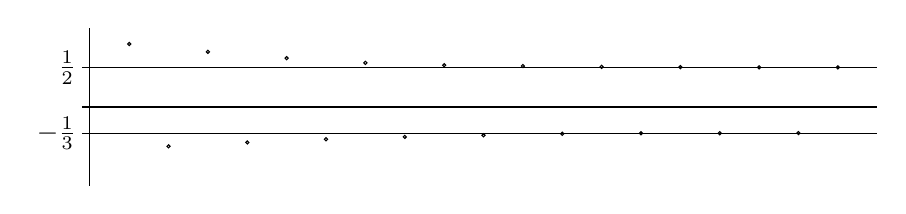
\begin{tikzpicture}
		\draw (0, -1) -- (0, 1);
		\draw (-0.1, 0) -- (10, 0);
		\draw[thin] (-0.1, 0.5) -- (10, 0.5);
		\draw[thin] (-0.1, -0.333) -- (10, -0.333);
		\draw (-0.05, -0.333) node[anchor = east] {$-\frac{1}{3}$} -- (0.05, -0.333);
		\draw (-0.05, 0.5) node[anchor = east] {$\frac{1}{2}$} -- (0.05, 0.5);
		\draw (0.5, 0.8) circle (0.02);
		\draw (1.5, 0.7) circle (0.02);
		\draw (2.5, 0.62) circle (0.02);
		\draw (3.5, 0.56) circle (0.02);
		\draw (4.5, 0.53) circle (0.02);
		\draw (5.5, 0.52) circle (0.02);
		\draw (6.5, 0.51) circle (0.02);
		\draw (7.5, 0.505) circle (0.02);
		\draw (8.5, 0.503) circle (0.02);
		\draw (9.5, 0.502) circle (0.02);
		\draw (1, -0.5) circle (0.02);
		\draw (2, -0.45) circle (0.02);
		\draw (3, -0.41) circle (0.02);
		\draw (4, -0.38) circle (0.02);
		\draw (5, -0.36) circle (0.02);
		\draw (6, -0.34) circle (0.02);
		\draw (7, -0.335) circle (0.02);
		\draw (8, -0.333) circle (0.02);
		\draw (9, -0.332) circle (0.02);
	\end{tikzpicture}
\end{subexample}

\begin{subtheorem}[Bolzano Weierstraß]
	Jede beschränkte Folge in $ \R $ besitzt eine konvergente Teilfolge.
\end{subtheorem}
\begin{sublemma}
	Jede Folge in $\R$ hat eine monotone Teilfolge.
\end{sublemma}
\begin{subproof*}
	Sei $ (a_n) \subset \R $ beschränkt. Nach Lem \ref{4.2.7} gibt es eine monotone Teilfolge, die natürlich auch beschränkt ist. Nach dem Satz über monotone, beschränkte Folgen konvergiert diese Teilfolge.\qed
\end{subproof*}
Brauchen:
\begin{subproof*}
	Sei $ (a_n) \subset \R $ bel. Wir nennen $ a_{n_0} (n_0 \in \N)$ \textbf{Gipfelpunkt}, falls:
	\begin{enumerate}[label=(\roman*)]
		\item \textbf{unendlich viele Gipfelpunkte}: Sei dann $ (a_{n_k}) $ Teilfolge der Gipfelpunkte.
			Dann \[ n_1 \leq n_2 \leq n_3 \leq \dotsb \text{ und} \]
			\[ a_{n_1} \geq a_{n_2} \geq a_{n_3} \geq \dotsb \]
			Also ist $ (a_{n_k}) $ monoton fallend.
		\item \textbf{endlich viele oder keine Gipfelpunkte:} Hier existiert
			\[ N \in \N : n \geq N \implies a_n \] kein Gipfelpunkt. Also gilt nicht:
			D. h. $ \exists n_1 \geq N: a_N < a_{n_1} \implies a_{n_1} $ kein Gipfelpunkt $\implies \exists N_2 \gneqq n_1 : a_{n_1} < a_{n_2}$, usf. Dann ist $ (a_{n_k} ) $ monoton wachsend.\qed
	\end{enumerate}
\end{subproof*}

\subsection{Charakterisierung der Vollständigkeit}
Für $ a \leq b $ sei $ [a, b] \coloneqq \{ x \in \R : a \leq x \leq b \} $. Der Durchmesser von $ [ a, b ] : \operatorname{diam}([a, b]) = b - a $

\begin{sublemma}
	Sei $ (a_n) $ Cauchyfolge, die eine gegen $ a\in \R $ konvergiente Teilfolge besitzt. Dann konvergiert $ (a_n ) $ gegen $ a $.
	\begin{subproof*}
		$\forall\varepsilon > 0 \exists N \in \N \forall n, m \geq N : | a_n - a_m | < \frac{\varepsilon}{2} $. Wähle zu $ \varepsilon > 0 $ ein solches $ N \in \N $.
		Dann gibt es wegen konvergenter Teilfolge einen Index $ \widetilde{N} \geq N : | a - a_{widetilde{N}} | < \frac{varepsilon}{2}$.
		Dann $ \forall n \geq N : $
		\begin{align*}
			| a_n - a | &= | ( a_n - a_{\widetilde{N}} ) + ( a_{\widetilde{N}} - a ) |\\
			&< \underbrace{a_n - a_{\widetilde{N}}|}_{\frac{\varepsilon}{2}} + \underbrace{a_{\widetilde{N}} - a|}_{\frac{\varepsilon}{2}} < \varepsilon
		\end{align*}
	\end{subproof*}
\end{sublemma}

\begin{subtheorem}
	Die folgenden Prinzipien sind auf $ \R $ äquivalent:
	\begin{enumerate}[label=(\roman*)]
		\item \textbf{Supremumseigenschaft:} Jede nichtleere, nach oben beschrenkte Menge hat ein Supremum.
		\item \textbf{Bolzano-Weierstraß-Eigenschaft:} Jede beschränkte Folge hat eine konvergente Teilfolge
		\item \textbf{Vollständigkeit:} Jede Cauchyfolge konvergiert
		\item \textbf{Intervallscachtelungsprinzip:} Sind $ (a_n), (b_n) \subset \R $ mit $ \forall n \in \N : a_n \leq b_n \wedge [a_{n+1}, b_{n+1}] \subset [a_n, b_n] $ mit
			$\lim_{n\to\infty} \operatorname{diam}([a_n, b_n]) = 0 $, so \textbf{existiert genau ein}
			\[ x \in \bigcap_{n\in\N}[a_n, b_n]. \]
	\end{enumerate}
	\begin{subproof*}
		Plan: $ (i) \implies (ii) \implies (iii) \implies (iv) \implies (i) $
		\begin{description}
			\item[Ad $ (i) \implies (ii) $] Die Supremumseigenschaft ist die einizige Zutat, um Bolzano-Weierstraß zu zeigen. Damit folgt $(ii)$ aus $(i)$
			\item[Ad $ (ii) \implies (iii) $] Sei $ (a_n) $ Cauchyfolge. Nach letzter Vorlesung ist $ ( a_n ) $ beschränkt, und nach $ (ii) $ hat $ (a_n ) $ also konvergiert Teilfolge. Nach Lem \ref{4.3.1} konvergiert dann aber bereits $ (a_n) \implies (iii) $
			\item[Ad $ (iii) \implies (iv)$] Sei $ ([a_n, b_n]) $ eine \textbf{Intervallschachtelung} mit $ \operatorname{diam}([a_n, b_n]) \to 0, n \to \infty. $. Sei $ \varepsilon > 0 $.
				Dann \[ \exists N \in \N : \forall n \geq N : \underbrace{\operatorname{diam}([a_n, b_n])}_{b_n - a_n} < \varepsilon \].
				Dann $ \forall n, m \geq N : a_m \in [a_n, b_n] $ (da Intervallschachtellung), also:
				\[ | a_n - a_m | \leq | a_n - b_n| < \varepsilon \implies (a_n) \textbf{ Cauchy}.\]
				Ähnlich: $ (b_n) \text{Cauchy} \overset{(iii)}{\implies} \exists a, b \in \R: a_n \to a, b_n \to b $.
				\[ | a- b| = \lim_{n\to\infty} \underbrace{|a_n -b_n}_{\operatorname{diam}([a_n, b_n])} = 0 \implies a = b. \]
				Kurz zu
				\[ a \in \bigcap_{n\in\N}[a_n, b_n] : (a_n) \text{ monoton wachsend}, (b_n) \text{ monoton fallend} \]
				\begin{align*}
					&\overset{\text{Stabilität der KG-Relation}}{\implies}
					\begin{drcases}
						a_1 \leq a_2 \leq \dotsb \leq a\\
						b  \geq \dotsb \geq b_2 \geq b_1
					\end{drcases}\\
					&\implies a_1 \leq a_2 \leq \dotsb \leq a = b \leq \dotsb \leq b_2 \leq b
				\end{align*}
				hier fehlt noch was ...
		\end{description}
	\end{subproof*}
\end{subtheorem}

\begin{subexample*}[einfach Beispiel aus Vorlesung]
	Ich glaube das soll zeigen, dass irgendwas an $ \R $ besonders
	\[ [ \sqrt{2} - 1, \sqrt{2} + \frac{1}{n} ] \]
	\[ \sqrt{2} - \frac{2}{n} \leq a_n leq \sqrt{2} - \frac{1}{n} \]
	\[ \sqrt{2} + \frac{1}{n} \leq b_n leq \sqrt{2} + \frac{1}{n} \]
	\[ [ a_n, b_n ], a_n, b_n \in \Q \]
\end{subexample*}



\end{document}
